Utilizing the knowledge of geometric transformations and projective geometries, a model of a camera can be systematically constructed step by step.
The reference frame is standardized, with the $z$ direction along the focal direction of the camera, the $x$ direction to the right, and the $y$ direction such that the right-hand rule is maintained.
The origin is at the center of the camera.

The object of interest is described as a collection of points, $\mathbf{p}_i =  [x_i, y_i, z_i, 1] \text{ for } i = 1,2,\cdots,N$.
In practice, all operations are uniformly performed on all points.
For clarity, the subsequent equations will illustrate the process using a single point of the object.

The first step is describing the location and orientation of the object with respect to the camera.
This rotation and translation can be captured using a single 3D homogenous transformation matrix (\cref{eq:4x4-homog-transformation}).

\begin{equation}
    \tilde{\mathbf{p}}' = \begin{bmatrix}
        \mathbf{R}_{3 \times 3} & \mathbf{t}_{3 \times 1} \\ \mathbf{0}_{1 \times 3} & 1
    \end{bmatrix} \tilde{\mathbf{p}}
    \label{eq:4x4-homog-transformation}
\end{equation}

Then, a projective transform is applied to each point in the object, controlling for the relative size and scaling based on the focal distance.
Geometrically, this relationship can be visualized with similar triangles (\cref{fig:perspective-projection}) and quantified using the ratio of lengths (\cref{eq:perspective-projection}).
In these equations, $f'$ is the focal distance in units of length.

\begin{figure}[h!]
    \begin{center}
        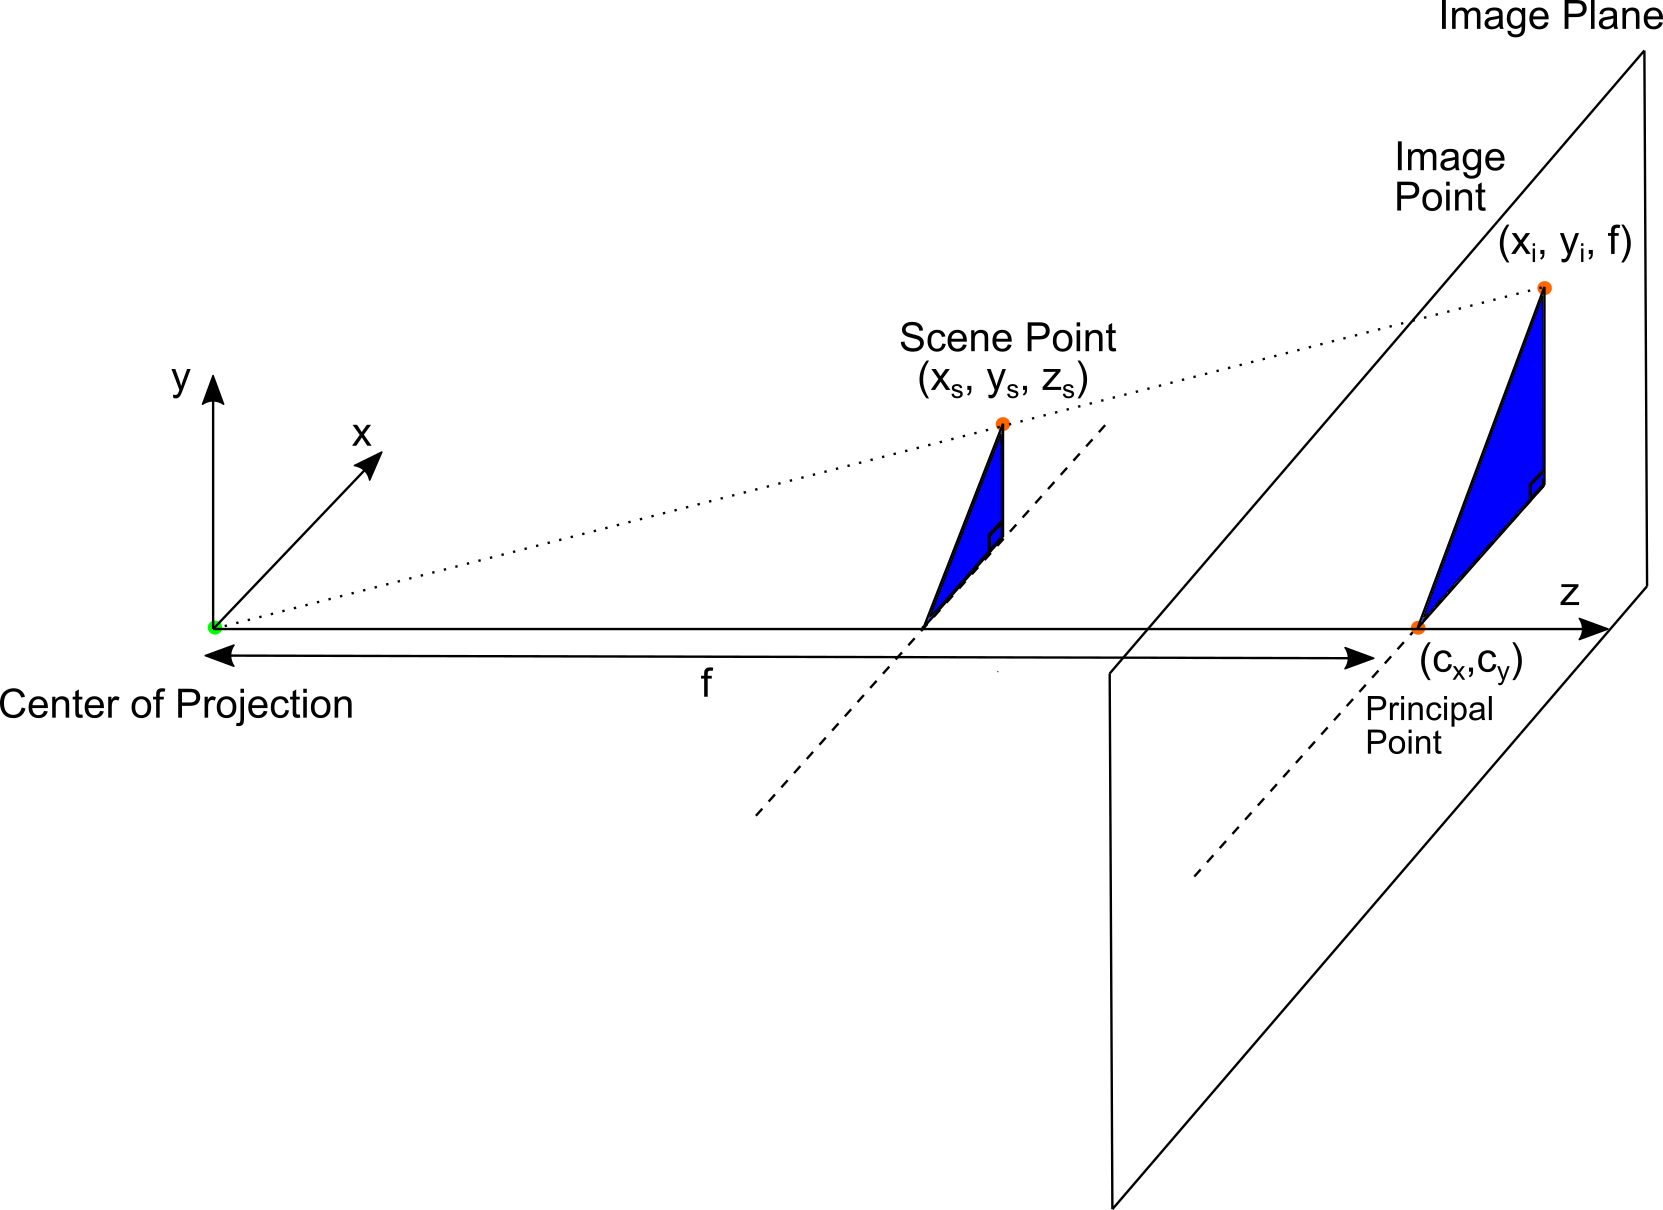
\includegraphics[width=0.85\linewidth]{figs/background/png/perspective-projection.png}
    \end{center}
    \caption{The geometry of perspective projection can be visualized by using similar triangles. The overall scaling of the image is based on the ratio of the focal length to the depth of the object.                                                 }
    \label{fig:perspective-projection}
\end{figure}


\begin{equation}
    \begin{aligned}
        \tilde{\mathbf{x}}_{i} &= \begin{bmatrix}
            f' & 0 & 0 \\ 0 & f' & 0 \\ 0 & 0 & 1 
        \end{bmatrix} \tilde{\mathbf{p}}' \\
        &\text{where} \\
        x_i &= p_x'\frac{f'}{p_z'} \\
        y_i &= p_y'\frac{f'}{p_z'} \\
    \end{aligned}
    \label{eq:perspective-projection}
\end{equation}

The standard image reference frame places the origin at the top left corner of the image, with the positive x-direction to the right, and the positive y-direction down.
This introduces the idea of the principal point, $(c_x,c_y)$, which is the location where the optical axis of the camera intersects the image plane perpendicularly.
In the camera model, the principal point is a translation starting at the image plane's origin (Eq. \ref{eq:principal-point}).



\begin{equation}
    \begin{aligned}
        \tilde{\mathbf{x}}_{i} &= \begin{bmatrix}
            f' & 0 & c_x \\ 0 & f' & c_y \\ 0 & 0 & 1 
        \end{bmatrix} \tilde{\mathbf{p}}' \\
        &\text{where} \\
        c_x &\approx \frac{W_{image}}{2} \\
        c_y &\approx \frac{H_{image}}{2} \\
    \end{aligned}
    \label{eq:principal-point}
\end{equation}


Lastly, the image coordinates, $\tilde{\mathbf{x}}_{i}$ must be converted to pixel coordinates using the pixel scaling factor.
The pixel scale factor is defined by the parameters $k_x$ and $k_y$, which represent the number of pixels per unit distance in the x and y directions, respectively.
Multiplying the perspective projection matrix by the pixel scale factor yields a new matrix that maps 3D points in ``world coordinates'' directly to pixel coordinates in the image.
\begin{equation}
    \begin{aligned}
        \tilde{\mathbf{x}}_{pix} &= \begin{bmatrix}
            k_x & 0& 0 \\ 0 & k_y & 0 \\ 0 & 0 & 1
        \end{bmatrix} \begin{bmatrix}
            f' & 0 & c_x \\ 0 & f' & c_y \\ 0 & 0 & 1 
        \end{bmatrix}\tilde{\mathbf{p}}' \\
        & = \begin{bmatrix}
            f_x & 0 & c_x \\ 0 & f_y & c_y \\ 0 & 0 & 1 
        \end{bmatrix}\tilde{\mathbf{p}}'\\
        &\text{where}\\
        f_x &= k_x f' \text{        and        } f_y = k_y f' \\
        &\text{Are focal distances in units of pixels} 
    \end{aligned}
    \label{eq:pixel-scaling}
\end{equation}


To generate a simple binary rasterization of the image, the space between projected points is interpolated and filled in, resulting in a binary "shadow" of the object on the image plane.
While more comprehensive image formation entails coloring, shading, and ray tracing, such complexity is unnecessary for the purpose of model-image registration of implant geometries in fluoroscopic images, and thus will not be addressed.

%%% Local Variables:
%%% mode: latex
%%% TeX-master: "../../../Andrew_Jensen_Dissertation"
%%% End:
